\documentclass[border=2mm]{standalone}
\usepackage{tikz}
\usetikzlibrary{positioning,fit,arrows.meta}

\begin{document}

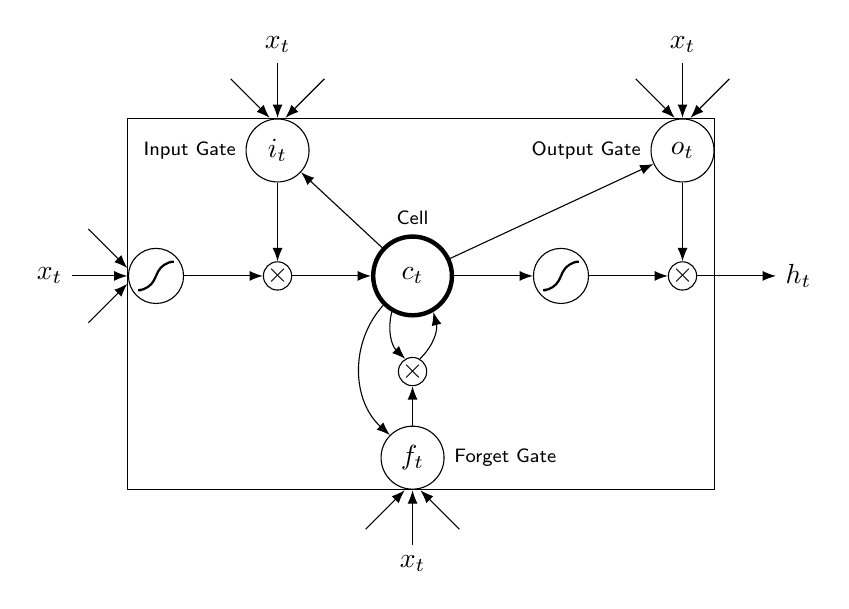
\begin{tikzpicture}[
    prod/.style={circle, draw, inner sep=0pt},
    ct/.style={circle, draw, inner sep=5pt, ultra thick, minimum width=10mm},
    ft/.style={circle, draw, minimum width=8mm, inner sep=1pt},
    filter/.style={circle, draw, minimum width=7mm, inner sep=1pt, path picture={\draw[thick, rounded corners] (path picture bounding box.center)--++(65:2mm)--++(0:1mm);
    \draw[thick, rounded corners] (path picture bounding box.center)--++(245:2mm)--++(180:1mm);}},
    mylabel/.style={font=\scriptsize\sffamily},
    >=LaTeX
    ]

\node[ct, label={[mylabel]Cell}] (ct) {$c_t$};
\node[filter, right=of ct] (int1) {};
\node[prod, right=of int1] (x1) {$\times$}; 
\node[right=of x1] (ht) {$h_t$};
\node[prod, left=of ct] (x2) {$\times$}; 
\node[filter, left=of x2] (int2) {};
\node[prod, below=5mm of ct] (x3) {$\times$}; 
\node[ft, below=5mm of x3, label={[mylabel]right:Forget Gate}] (ft) {$f_t$};
\node[ft, above=of x2, label={[mylabel]left:Input Gate}] (it) {$i_t$};
\node[ft, above=of x1, label={[mylabel]left:Output Gate}] (ot) {$o_t$};

\foreach \i/\j in {int2/x2, x2/ct, ct/int1, int1/x1,
            x1/ht, it/x2, ct/it, ct/ot, ot/x1, ft/x3}
    \draw[->] (\i)--(\j);

\draw[->] (ct) to[bend right=45] (ft);

\draw[->] (ct) to[bend right=30] (x3);
\draw[->] (x3) to[bend right=30] (ct);

\node[fit=(int2) (it) (ot) (ft), draw, inner sep=0pt] (fit) {};

\draw[<-] (fit.west|-int2) coordinate (aux)--++(180:7mm) node[left]{$x_t$};
\draw[<-] ([yshift=1mm]aux)--++(135:7mm);
\draw[<-] ([yshift=-1mm]aux)--++(-135:7mm);

\draw[<-] (fit.north-|it) coordinate (aux)--++(90:7mm) node[above]{$x_t$};
\draw[<-] ([xshift=1mm]aux)--++(45:7mm);
\draw[<-] ([xshift=-1mm]aux)--++(135:7mm);

\draw[<-] (fit.north-|ot) coordinate (aux)--++(90:7mm) node[above]{$x_t$};
\draw[<-] ([xshift=1mm]aux)--++(45:7mm);
\draw[<-] ([xshift=-1mm]aux)--++(135:7mm);

\draw[<-] (fit.south-|ft) coordinate (aux)--++(-90:7mm) node[below]{$x_t$};
\draw[<-] ([xshift=1mm]aux)--++(-45:7mm);
\draw[<-] ([xshift=-1mm]aux)--++(-135:7mm);
\end{tikzpicture}
\end{document}